% Foliensatz: "AFu-Kurs nach DJ4UF" von DK0TU, Amateurfunkgruppe der TU Berlin
% Lizenz: CC BY-NC-SA 3.0 de (http://creativecommons.org/licenses/by-nc-sa/3.0/de/)
% Autoren: Felix Baum <baum@campus.tu-berlin.de>
% Korrekturen: Lars Weiler <dc4lw@darc.de>, Sebastian Lange <dl7bst@dk0tu.de>

\documentclass[aspectratio=169]{beamer}

\usepackage[ngerman]{babel} % deutsche Worttrennung etc.
\usepackage[utf8]{inputenc} % UTF8 Text

\usepackage[super, comma, numbers, square, sort]{natbib}

\usepackage{hyperref}       % Hyperref Package für bessere Referenzen (todo)
\hypersetup{
	colorlinks=false,       %   false: boxed links; true: colored links
    %linkcolor=white,       %   color of internal links (change box color with linkbordercolor)
    citecolor=red,          %   color of links to bibliography
    filecolor=white,        %   color of file links
    urlcolor=blue           %   color of external links
}

\usepackage{multirow}
\usepackage{wasysym}  % Math Symbols like \permil
%\usepackage{colortbl}
%\usepackage{subscript}
%\usepackage{caption}
%\usepackage{setspace}
%\usepackage{xcolor}        % benutze CodeListe

% Footnote
%\usepackage{hanging}
%
%\setbeamertemplate{footnote}{%
%  \hangpara{2em}{1}%
%  \makebox[2em][l]{\insertfootnotemark}\footnotesize\insertfootnotetext\par%
%}


%\usepackage{pgf}
%\usepackage{tikz}
%\usetikzlibrary{arrows,automata}
%\usetikzlibrary{positioning}
%
%\tikzset{
%    state/.style={
%           rectangle,
%           rounded corners,
%           draw=black, very thick,
%           minimum height=2em,
%           minimum width=2pt,
%           inner sep=2pt,
%           text centered,
%           },
%}

%\usepackage{listings}
%\lstset{basicstyle=\small, numberstyle=\tiny, extendedchars=true, numbers=left, numbersep=5pt}
%\lstset{showtabs=false, showspaces=false, showstringspaces=false}
%%\lstset{backgroundcolor=\color{white!75!lightgray}, , frame=single}
%%\lstset{backgroundcolor=\color{white}}
%%\lstset{backgroundcolor=none}
%\lstset{keywordstyle=\color{blue!50!gray},  identifierstyle=\color{black}}
%\lstset{commentstyle=\color{green!50!gray}, stringstyle=\color{red!50!gray}}
%\lstset{language=C, fontadjust=true, tabsize=2, breaklines=true}
%\lstset{backgroundcolor=\color{white!75!lightgray}, caption=\lstname, frame=single}
%\lstset{emphstyle=\color{black}\fbox}
%
%% Keine "Listing:"-Caption
%\captionsetup{labelformat=empty,labelsep=none}
%
%% für mathematische Umgebungen
%\usepackage{amsmath,amsfonts,amssymb}
%
%\lstdefinestyle{Bash}{
%language=Bash,
%frame=single,
%rulecolor=\color{black},
%backgroundcolor=\color{gray!50},
%keywordstyle=\color{black},
%identifierstyle=,
%commentstyle=\color{black},
%stringstyle=\color{magenta!65!white},
%showstringspaces=false,
%basicstyle=\footnotesize\ttfamily\color{black},
%numbers=none,
%breaklines=true,
%captionpos=b
%}

%\usepackage{listings}
%
%\lstdefinestyle{basic}{
%    captionpos=t,%
%    basicstyle=\footnotesize\ttfamily,%
%    numberstyle=\tiny,%
%    numbers=left,%
%    stepnumber=1,%
%    frame=single,%
%    showspaces=false,%
%    showstringspaces=false,%
%    showtabs=false,%
%    %
%    keywordstyle=\color{blue},%
%    identifierstyle=,%
%    commentstyle=\color{gray},%
%    stringstyle=\color{magenta}%
%}



% fließende Boxen haben keinen Abstand
%\fboxsep0mm

% inkludiere Creative Commons Helper
%%%%%%%%%%%%%%%%%%%%%%%%%%%%%%%%%%%%%%%%%%%%%%%%%%%%%%%%%%%%%%%%
%% ccBeamer 0.1, 2007-07-02                                   %%
%% Written by Sebastian Pipping <webmaster@hartwork.org>      %%
%% ---------------------------------------------------------- %%
%% Licensed under Creative Commons Attribution-ShareAlike 3.0 %%
%% http://creativecommons.org/licenses/by-sa/3.0/             %%
%%%%%%%%%%%%%%%%%%%%%%%%%%%%%%%%%%%%%%%%%%%%%%%%%%%%%%%%%%%%%%%%


%% Images
\newcommand{\CcImageBy}[1]{%
	
\includegraphics[scale=#1]{texdata/creative_commons/cc_by_30.pdf}%
}
\newcommand{\CcImageCc}[1]{%
	
\includegraphics[scale=#1]{texdata/creative_commons/cc_cc_30.pdf}%
}
\newcommand{\CcImageDevNations}[1]{%
	
\includegraphics[scale=#1]{texdata/creative_commons/cc_dev_nations_30.pdf}%
}
\newcommand{\CcImageNc}[1]{%
	
\includegraphics[scale=#1]{texdata/creative_commons/cc_nc_30.pdf}%
}
\newcommand{\CcImageNd}[1]{%
	
\includegraphics[scale=#1]{texdata/creative_commons/cc_nd_30.pdf}%
}
\newcommand{\CcImagePd}[1]{%
	
\includegraphics[scale=#1]{texdata/creative_commons/cc_pd_30.pdf}%
}
\newcommand{\CcImageSa}[1]{%
	
\includegraphics[scale=#1]{texdata/creative_commons/cc_sa_30.pdf}%
}
\newcommand{\CcImageSampling}[1]{%
	
\includegraphics[scale=#1]{texdata/creative_commons/cc_sampling_30.pdf}%
}
\newcommand{\CcImageSamplingPlus}[1]{%
	
\includegraphics[scale=#1]{texdata/creative_commons/cc_sampling_plus_30.pdf}%
}


%% Groups
\newcommand{\CcGroupBy}[2]{% zoom, gap
	\CcImageCc{#1}\hspace*{#2}\CcImageBy{#1}%
}
\newcommand{\CcGroupByNc}[2]{% zoom, gap
	\CcImageCc{#1}\hspace*{#2}\CcImageBy{#1}\hspace*{#2}\CcImageNc{#1}%
}
\newcommand{\CcGroupByNcNd}[2]{% zoom, gap
	\CcImageCc{#1}\hspace*{#2}\CcImageBy{#1}\hspace*{#2}\CcImageNc{#1}\hspace*{#2}\CcImageNd{#1}%
}
\newcommand{\CcGroupByNcSa}[2]{% zoom, gap
	\CcImageCc{#1}\hspace*{#2}\CcImageBy{#1}\hspace*{#2}\CcImageNc{#1}\hspace*{#2}\CcImageSa{#1}%
}
\newcommand{\CcGroupByNd}[2]{% zoom, gap
	\CcImageCc{#1}\hspace*{#2}\CcImageBy{#1}\hspace*{#2}\CcImageNd{#1}%
}
\newcommand{\CcGroupBySa}[2]{% zoom, gap
	\CcImageCc{#1}\hspace*{#2}\CcImageBy{#1}\hspace*{#2}\CcImageSa{#1}%
}
\newcommand{\CcGroupDevNations}[2]{% zoom, gap
	\CcImageCc{#1}\hspace*{#2}\CcImageDevNations{#1}%
}
\newcommand{\CcGroupNcSampling}[2]{% zoom, gap
	\CcImageCc{#1}\hspace*{#2}\CcImageNc{#1}\hspace*{#2}\CcImageSampling{#1}%
}
\newcommand{\CcGroupPd}[1]{% zoom
	\CcImagePd{#1}%
}
\newcommand{\CcGroupSampling}[1]{% zoom
	\CcImageSampling{#1}%
}
\newcommand{\CcGroupSamplingPlus}[1]{% zoom
	\CcImageSamplingPlus{#1}%
}


%% Text
\newcommand{\CcLongnameBy}{Attribution}
\newcommand{\CcLongnameByNc}{Attribution-NonCommercial}
\newcommand{\CcLongnameByNcNd}{Attribution-NoDerivs}
\newcommand{\CcLongnameByNcSa}{Attribution-NonCommercial-ShareAlike}
\newcommand{\CcLongnameByNd}{Attribution-NoDerivs}
\newcommand{\CcLongnameBySa}{Attribution-ShareAlike}

\newcommand{\CcNote}[1]{% longname
	This work is licensed under the \textit{Creative Commons #1 3.0 License}.%
}


% generelles Thema auswählen
\usetheme{Goettingen} %Berlin spart ohne Sidebar allerdings angenehm Platz
% AnnArbor | Antibes | Bergen | Berkeley | Berlin | Boadilla | boxes | CambridgeUS | Copenhagen | Darmstadt | default | Dresden | Frankfurt | Goettingen | Hannover | Ilmenau | JuanLesPins | Luebeck | Madrid | Malmoe | Marburg | Montpellier | PaloAlto | Pittsburgh | Rochester | Singapore | Szeged | Warsaw

% Farben wählen
\usecolortheme{beetle}
% beaver | beetle | crane | default | dolphin | dove | fly | lily | orchid | rose | seagull | seahorse | sidebartab | structure | whale | wolverine

% Setze alle Farben auf Grau und Weiß
%\definecolor{craneorange}{RGB}{64,64,64}
%\definecolor{craneblue}{RGB}{255,255,255}

% Schriftart wählen
\usefonttheme{default}
% default | professionalfonts | serif | structurebold | structureitalicserif | structuresmallcapsserif

% Innere Themen(Kopf-, Fuß-, Sidebar usw)
%\useinnertheme{default}
\useinnertheme{circles}
% default | inmargin | rectangles | rounded | circles

% Äußere Themen (Anordnung der inneren, grenzen der Folien etc.)
\useoutertheme{infolines}
% default | infolines | miniframes | shadow | sidebar | smoothbars | smoothtree | split | tree

% Deaktiviere Navigations-Symbole ({} -> leer)
\setbeamertemplate{navigation symbols}{}
%\setbeamertemplate{navigation symbols}{\large \ifnum \insertframenumber <10 0\fi\insertframenumber/\inserttotalframenumber\vspace*{0.2ex}}

% Zeige ein Hintergrundbild
\setbeamertemplate{background canvas}{
        \hspace*{-2.0cm}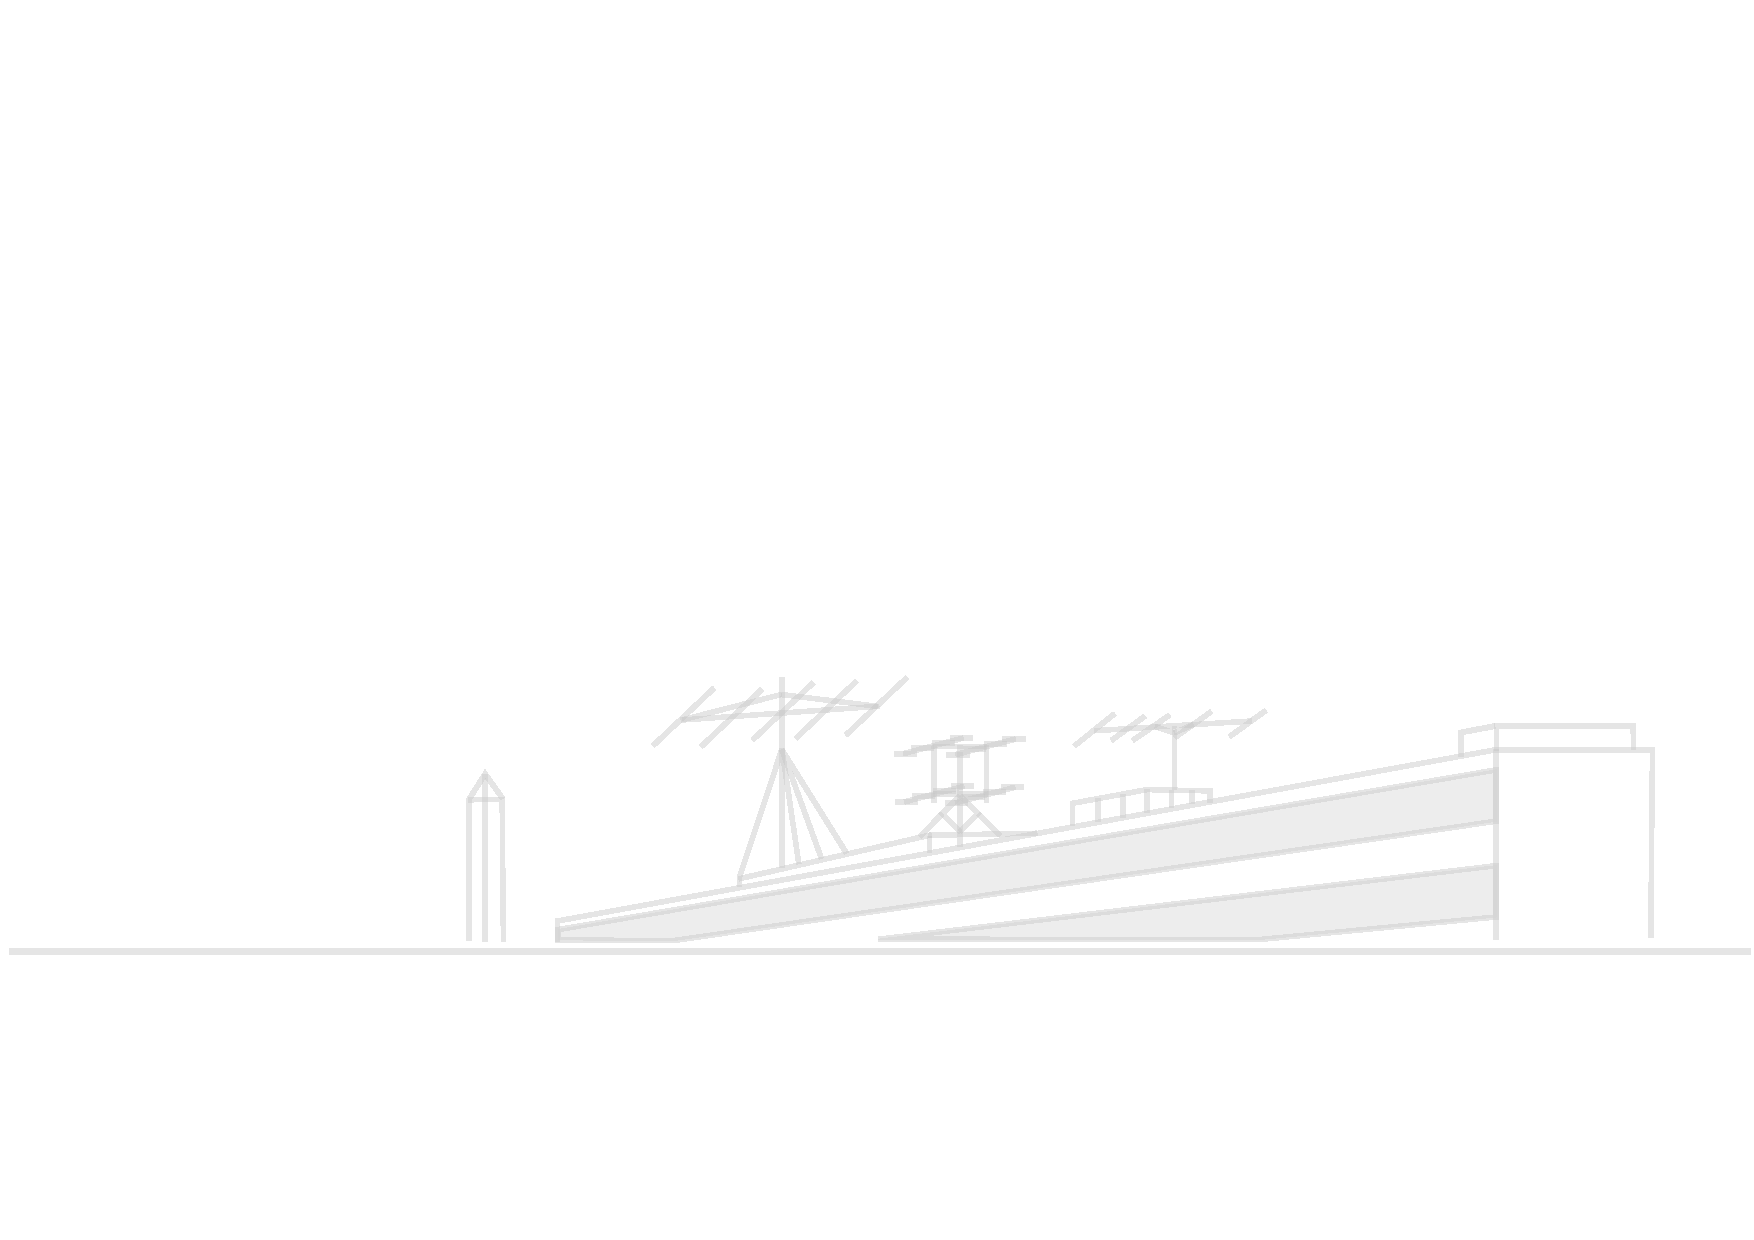
\includegraphics[width=17.8cm]{texdata/dk0tu_rooftop_background.pdf}
}

% Foliennummer einfügen
\setbeamertemplate{footline}[frame number]
%\setbeamertemplate{footline}{}

% Ändere das Zeichen vor jedem item
%\setbeamertemplate{itemize item}{\color{craneorange}$\blacktriangleright$}
%\setbeamertemplate{itemize subitem}{\color{craneorange}$\triangleright$}
%\setbeamertemplate{itemize subsubitem}{\color{craneorange}$\blacktriangleright$}

% Ändert die Blöcke 
\setbeamertemplate{blocks}[rounded][shadow=true]
% default | rounded [shadow=true|false]

%
% Eigene Kommandos
%

% Hack to get natbib and beamer working together. "The beamer user guide suggests
% that only the manual bibliography entry approach is supported"
% on some system it works out of the box, sometimes you need the hack :-(
% so check it --dl7bst
\ifdefined\newblock
    \relax
\else
    \newcommand{\newblock}{}
\fi

% \includedia command to generate png out of a dia file
% NEEDS installed dia and pdflatex option --shell-escape
\newcommand{\includedia}[1]{
    \immediate\write18{/usr/bin/dia #1.dia -e #1_diatmp.png -t png}
}

% RICHIG GROSSER FONT!
\newfont{\bigfont}{cmr10 at 144pt}
\newfont{\smallfont}{cmr10 at 8pt}

% Römische Ziffern
\makeatletter
\newcommand{\rmnum}[1]{\romannumeral #1}
\newcommand{\Rmnum}[1]{\expandafter\@slowromancap\romannumeral #1@}
\makeatother

% Schwarze Überschrift
%\setbeamercolor{frametitle}{fg=black}
%\setbeamercolor{title}{fg=black}

% Item- und Box-Farben
\definecolor{deepBlue}{HTML}{000066}
\setbeamercolor{itemize item}{fg=deepBlue}
\setbeamercolor{itemize subitem}{fg=deepBlue}
\setbeamercolor{description item}{fg=deepBlue}
\setbeamercolor{block title}{fg=deepBlue!100, bg=blue!15}
\setbeamercolor{block body}{fg=black, bg=blue!5}
\setbeamercolor{block title alerted}{fg=deepBlue, bg=red!75}
\setbeamercolor{block body alerted}{fg=black, bg=red!15}
\setbeamercolor*{block title example}{fg=blue!50, bg=blue!10}
\setbeamercolor*{block body example}{fg= blue, bg=blue!5}

%\setbeamercolor{section in head/foot}{parent=palette primary}
%\setbeamercolor{subsection in head/foot}{parent=palette secondary}
%\setbeamercolor{sidebar}{fg=darkblue,bg=yellow!90!orange}
%\setbeamercolor{title in sidebar}{fg=darkblue}
%\setbeamercolor{author in sidebar}{fg=darkblue}
%\setbeamercolor{section in sidebar}{fg=darkblue!10!black}
%\setbeamercolor{subsection in sidebar}{fg=darkblue!50!black}

% Titlepage Infos
\title{AFu-Kurs nach DJ4UF}
\author[DKØTU]{DKØTU\\ \footnotesize{Amateurfunkgruppe der TU Berlin}}
\institute[DKØTU]{\url{http://www.dk0tu.de} }

% PDF-Eigenschaften
\subject{DK0TU-Amateurfunkkurs nach DJ4UF}
\keywords{Amateurfunk Kurs HAM Radio Course CC-BY-NC-SA OpenSource TU Berlin DK0TU}

\subtitle{Technik Klasse E 06: \\
  Spule und Transformator \\[2em]}
\date{Stand 07.11.2016}
 \begin{document}

\begin{frame}
    \titlepage
    \vfill
    \begin{center}
        \ccbyncsaeu\\
        {\tiny This work is licensed under the \em{Creative Commons Attribution-NonCommercial-ShareAlike 3.0 License}.}\\[0.5ex]
         \tiny Amateurfunkgruppe der Technische Universität Berlin (AfuTUB), DKØTU
         %\includegraphics[scale=0.5]{img/DK0TU_Logo.pdf}
    \end{center}
\end{frame}



\section*{Einleitung}

\begin{frame}
  \frametitle{Einleitung / Spule}
  \begin{center}
    \Large{Wofür braucht man Spulen?} \\
  \end{center}
\end{frame}

\begin{frame}
  \frametitle{Diverse Anwendungsmöglichkeiten}
  \begin{itemize}
    \item Erzeugung von Magnetfeldern
    \item Detektion von Magnetfeldern
    \item Transformator
    \item Relais
    \item Elektromotor
    \item Lautsprecher
    \item Mikrofon
    \item LC-Schwingkreis
    \item Tief-, Hoch-, Bandpass
    \item Stromflussglättung
    \item Energiespeicher
    \item Drossel
    \item NFC, RFID-Transponder
  \end{itemize}
\end{frame}

\begin{frame}
  \frametitle{Einleitung / Spulen-Beispiele}
  \begin{center}
    \begin{figure}
      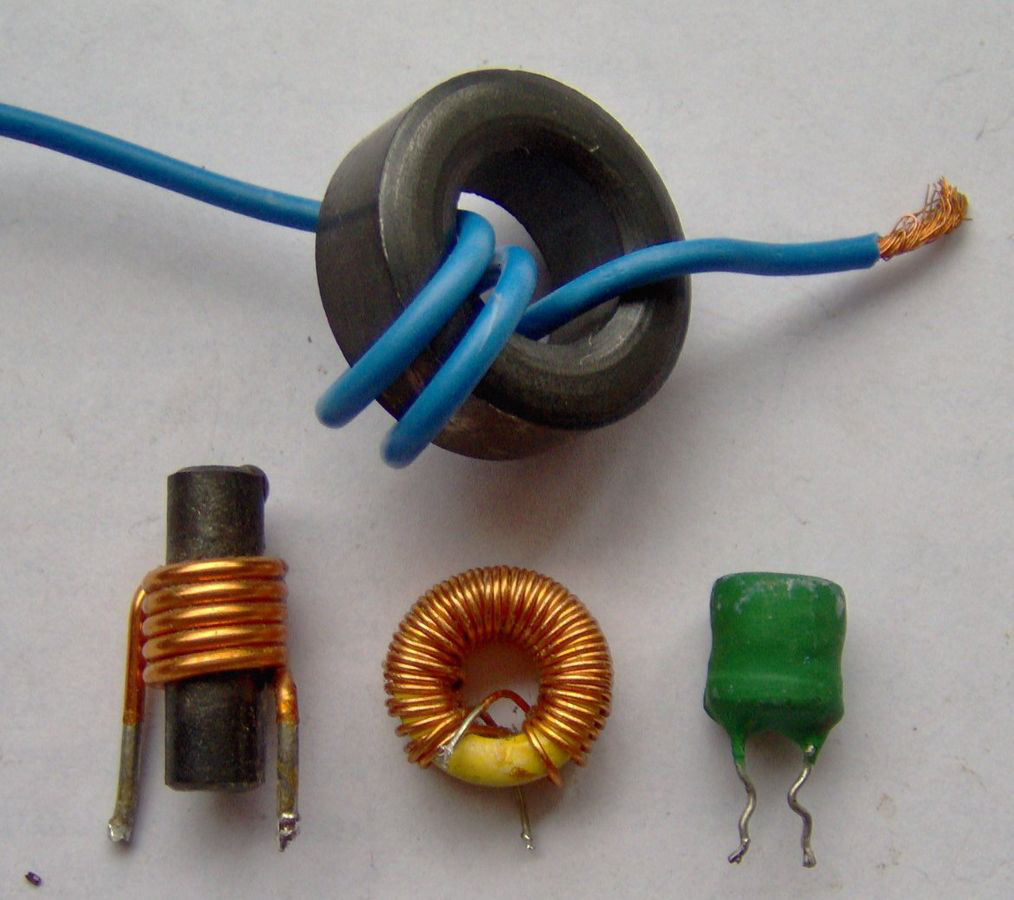
\includegraphics[height=0.75\textheight,width=\textwidth,keepaspectratio]{e06/Spule.jpg}
      \attribcaption{Spulen}{FDominec}{https://commons.wikimedia.org/wiki/File:Electronic_component_inductors.jpg}{\ccbysa}
    \end{figure}
  \end{center}
\end{frame}

\begin{frame}
  \frametitle{Einleitung / SMD-Spule}
  \begin{center}
    \begin{figure}
      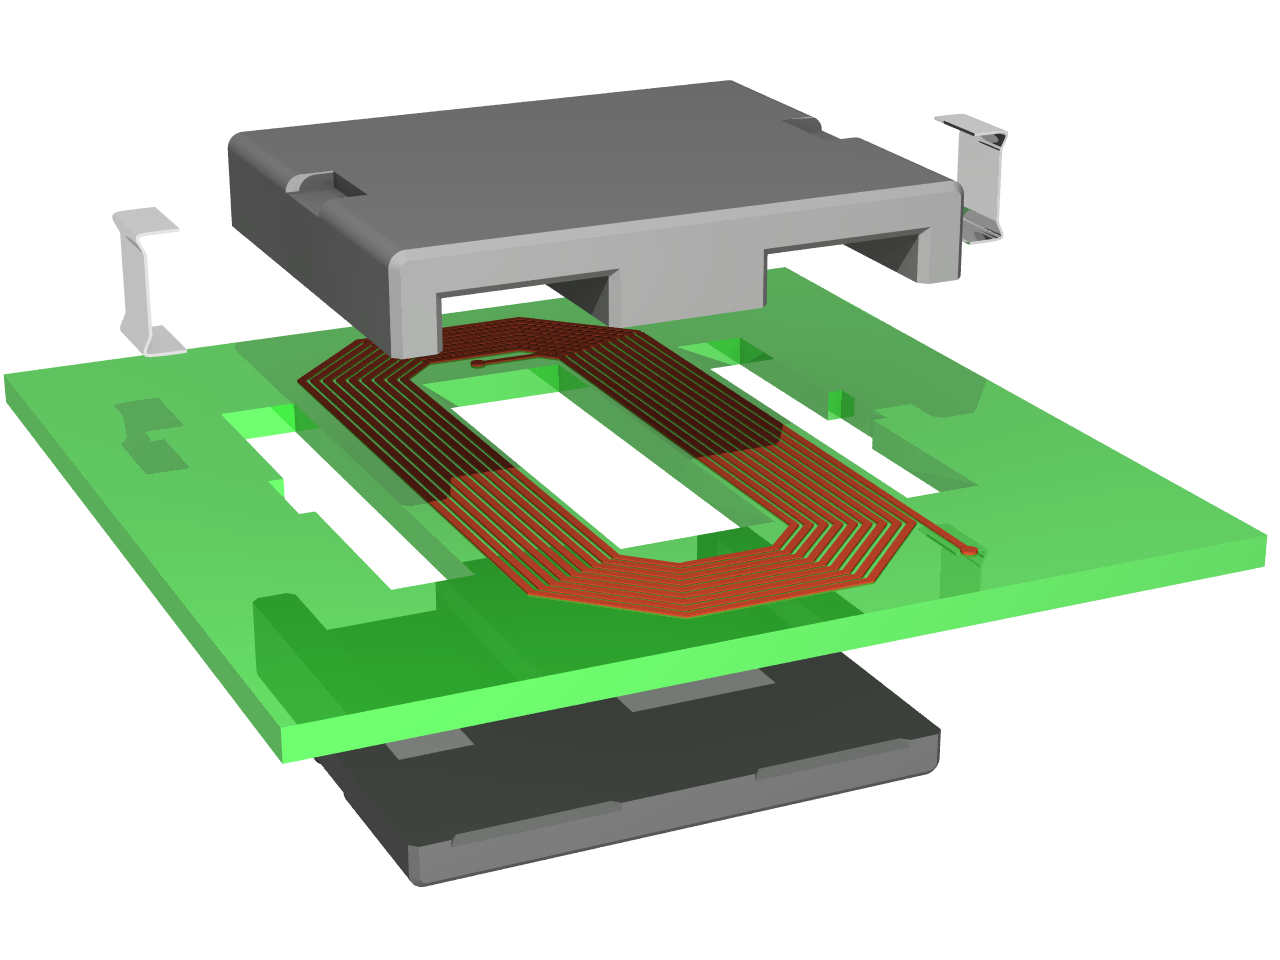
\includegraphics[height=0.75\textheight,width=\textwidth,keepaspectratio]{e06/smd-Spule.png}
      \attribcaption{Spule in SMD}{Cyril BUTTAY}{https://de.wikipedia.org/wiki/Datei:Planar_core_assembly_exploded.png}{\ccbysa}
    \end{figure}
  \end{center}
\end{frame}


% XXX von e08 übernommen, da es besser von der Reihenfolge passt
\section*{Induktivitäten}

\begin{frame}
  \frametitle{Das magnetische Feld}
  \begin{center}
    \begin{minipage}{0.45\textwidth}
      \begin{center}
        \begin{figure}
          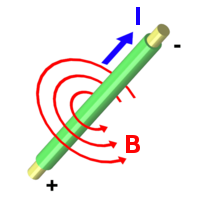
\includegraphics[width=\textwidth,height=.3\textheight,keepaspectratio]{e08/RechteHand.png}
          \attribcaption{Magnetisches Feld um einen Leiter}{Smial}{https://commons.wikimedia.org/wiki/File:RechteHand.png}{\ccbysa}
        \end{figure}
      \end{center}
    \end{minipage}
    \begin{minipage}{0.45\textwidth}
      \begin{center}
        \begin{figure}
          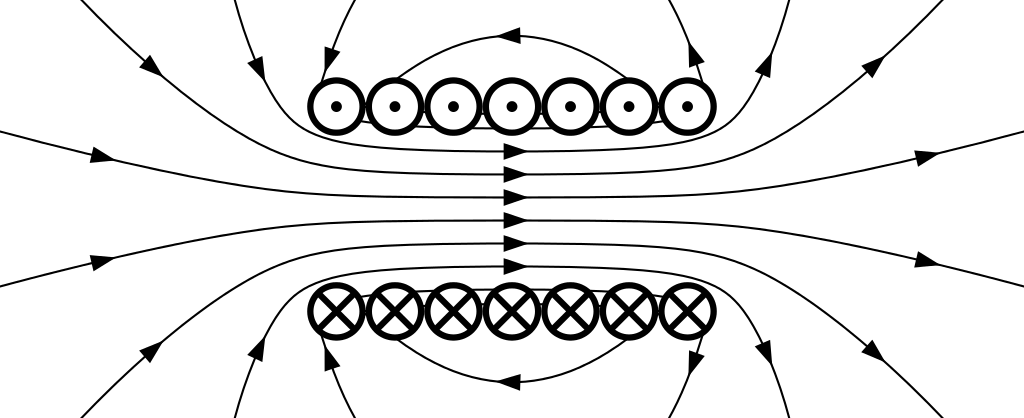
\includegraphics[width=\textwidth,height=.3\textheight,keepaspectratio]{e06/seopardy2.png}\\
          \attribcaption{Magnetisches Feld in einer Spule}{Geek3}{https://commons.wikimedia.org/wiki/File:VFPt_Solenoid_correct2.svg}{\ccbysa}
        \end{figure}
      \end{center}
    \end{minipage}
    \vspace{0.5cm}
    \begin{itemize}
      \item um jeden stromdurchflossenen Leiter baut sich ein konzentrisches, magnetisches Feld auf
      \item magnetische Felder summieren sich in einer Spule
      \item magnetische Felder in einer Spule sind homogen
      \item wird mit zunehmendem Strom stärker
      \item nimmt mit zunehmendem Abstand ab
    \end{itemize}
  \end{center}
\end{frame}

\begin{frame}
  \frametitle{3D Magnetisches Feld}
  \begin{center}
    \begin{figure}
      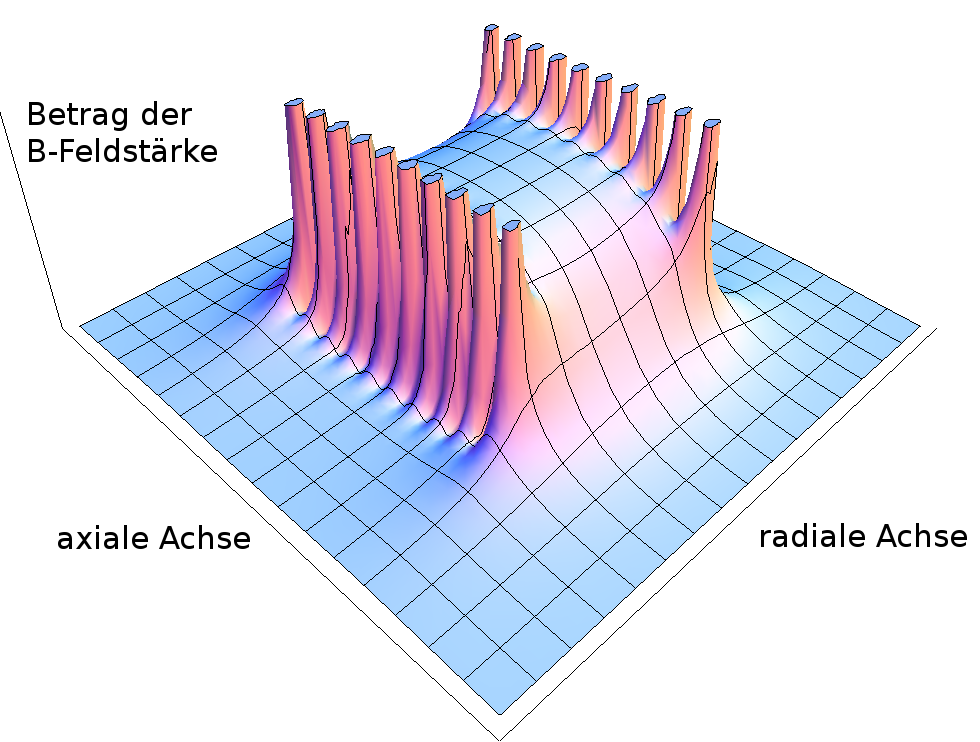
\includegraphics[width=1\textwidth,height=.75\textheight,keepaspectratio]{e06/3-D_HFeld.png}
      \attribcaption{Zeigt die B-Feldstärke als eine Funktion des Ortes in einer Zylinderspule mit zehn Windungen. Die Schnittebene geht durch das Zentrum in axialer Richtung.}{Tou-x}{https://commons.wikimedia.org/wiki/File:Solenoid.png}{\ccbysa}
    \end{figure}
  \end{center}
\end{frame}


\section*{Zylinderspule}

\begin{frame}
  \frametitle{Zylinderspule}
  \begin{center}
    \begin{figure}
      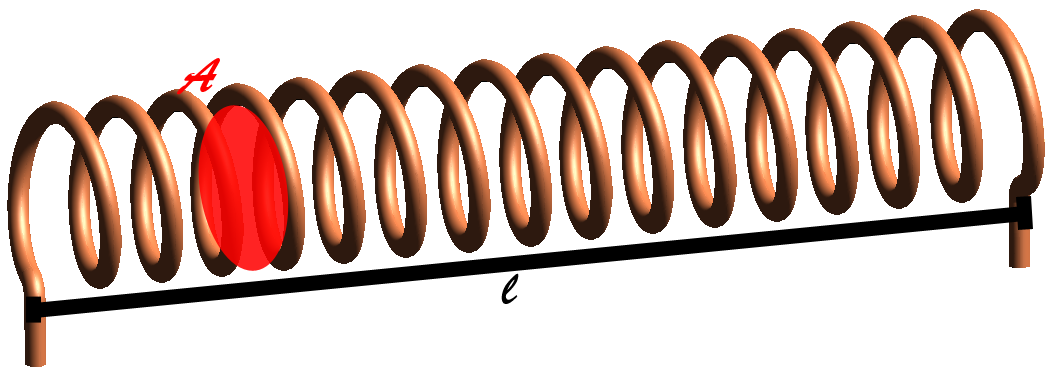
\includegraphics[width=1\textwidth]{e06/Luftspule.png}
      \caption{Luftspule}  % FIXME Quelle?
    \end{figure}
  \end{center}
\end{frame}

\begin{frame}
  \frametitle{Berechnung der Induktivität}
  \begin{block}{}
    \begin{center}
      \huge{$L = \cfrac{\mu \cdot A}{\ell_m}\cdot N^2$}\\[1em]
      \small{mit
      \begin{description}
        \item[$\mu$] $= \mu_0 \cdot \mu_r$
        \item[$\mu_{0}$] $= 1,25666 \cdot 10^{-6}\frac{H}{m}$: magnetische Feldkonstante
        \item[$\mu_{r}$] relative Permeabilität
        \item[$A$] Querschnitt der Spule
        \item[$N$] Windungszahl
        \item[$\ell_{m}$] mittlere Feldlinienlänge
      \end{description}
      }
    \end{center}
  \end{block}
\end{frame}

%\begin{frame}
%  \frametitle{Prüfungsfrage}
%  \begin{center}
%    \begin{tabular}{l||p{.8\textwidth}}
%      \textbf{TC302} & \textbf{Wie ändert sich die Induktivität einer Spule von $12 \mu H$ wenn die Wicklung auf dem  Wickelkörper bei gleicher Windungszahl auf den doppelten Wert auseinander gezogen wird?} \\\hline\hline
%      A & Die Induktivität sinkt auf $3 \mu H$. \\ \hline
%      B & Die Induktivität steigt auf $48 \mu H$. \\ \hline
%      C & Die Induktivität steigt auf $24 \mu H$. \\ \hline
%      D \only<2>\checkmark & Die Induktivität sinkt auf $6 \mu H$. \\ \hline
%    \end{tabular}
%  \end{center}
%\end{frame}
%
%\begin{frame}
%  \frametitle{Prüfungsfrage}
%  \begin{center}
%    \begin{tabular}{l||p{.8\textwidth}}
%      \textbf{TC303} & \textbf{Wie kann man die Induktivität einer Spule vergrößern?} \\\hline\hline
%      A & Durch Auseinanderziehen der Spule (Vergrößerung der Spulenlänge). \\ \hline
%      B \only<2>\checkmark & Durch Stauchen der Spule (Verkürzen der Spulenlänge). \\ \hline
%      C & Durch Einführen eines Kupferkerns in die Spule. \\ \hline
%      D & Durch Einbau der Spule in einen Abschirmbecher. \\ \hline
%    \end{tabular}
%  \end{center}
%\end{frame}


\section*{Wechsel\-strom\-kreis}

\begin{frame}
  \frametitle{Funktionsprinzip im Wechselstromkreis}
  \begin{columns}
    \column{0.3\textwidth}
    \begin{figure}
      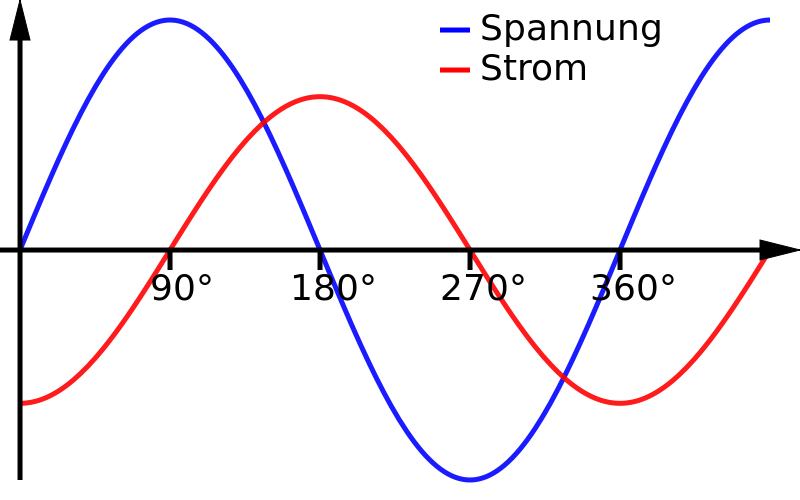
\includegraphics[width=1\textwidth,height=.75\textheight,keepaspectratio]{e06/800px-Phasenverschiebung_induktiv.png}
      \attribcaption{Phasverschiebung induktiv}{Hyperstryke}{https://commons.wikimedia.org/wiki/File:Phasenverschiebung_induktiv.svg}{\ccpd}
    \end{figure}
    \column{0.65\textwidth}
    {\small
    \begin{itemize}
      \item Magnetisches Feld wird ständig umgepolt
      \item Selbstinduktionsspannung entsteht
      \item Diese ist dem Strom entgegengerichtet
      \item Strom wird ``gebremst''
    \end{itemize}
    }
  \end{columns}
  \begin{block}{Merksatz}
    [Bei] Induktivitäten: Ströme sich verspäten
  \end{block}
\end{frame}

\begin{frame}
  \frametitle{Induktiver Widerstand}

  Abhängig von der Frequenz $f$.

  \begin{block}{Induktivität als Blindwiderstand}
    \begin{center}
      \huge{$X_L = 2 \cdot \pi \cdot f \cdot L$}
    \end{center}
  \end{block}

  \pause
  Der Blindwiderstand steigt bei zunehmender Frequenz.\\
  Der Blindwiderstand steigt bei größerer Induktivität.
\end{frame}

%\begin{frame}
%  \frametitle{Prüfungsfrage}
%  \begin{center}
%    \begin{tabular}{l||p{.8\textwidth}}\hline
%      \textbf{TC306} & \textbf{Mit zunehmender Frequenz} \\\hline\hline
%      A & sinkt der Wechselstromwiderstand der Spule bis zu einem Minimum und steigt dann wieder. \\ \hline
%      B & steigt der Wechselstromwiderstand der Spule bis zu einem Maximum und sinkt dann wieder. \\ \hline
%      C \only<2>\checkmark & steigt der Wechselstromwiderstand der Spule. \\ \hline
%      D & sinkt der Wechselstromwiderstand der Spule. \\ \hline
%    \end{tabular}
%  \end{center}
%\end{frame}


\section*{Schaltungen mit Spulen}

\begin{frame}
  \frametitle{Schaltzeichen}
  \begin{center}
    \begin{figure}
      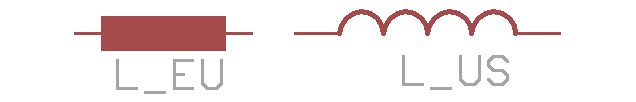
\includegraphics[width=1\textwidth,height=.75\textheight,keepaspectratio]{e06/Spule-schaltZ.png}
      \caption{Schaltzeichen einer Spule}
    \end{figure}
  \end{center}
\end{frame}


\subsection*{Reihen\-schaltung}

\begin{frame}
  \frametitle{Reihenschaltung}
  \begin{center}
    \begin{figure}
      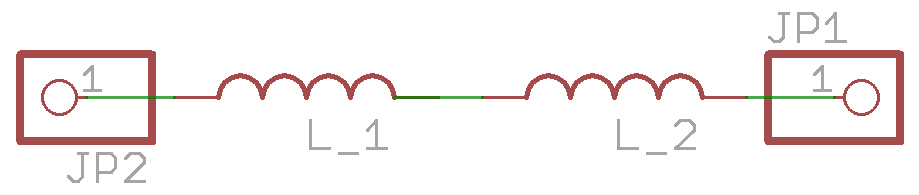
\includegraphics[width=1\textwidth,height=.5\textheight,keepaspectratio]{e06/L_Reihe.png}
      \caption{Spulen in einer Reihenschaltung}
    \end{figure}
  \end{center}
  \begin{block}{Reihenschaltung}
    $L_{gesamt} = L_1 + L_2 + L_3 + ...$
  \end{block}
\end{frame}


\subsection*{Parallel\-schaltung}

\begin{frame}
  \frametitle{Parallelschaltung}
  \begin{center}
    \begin{figure}
      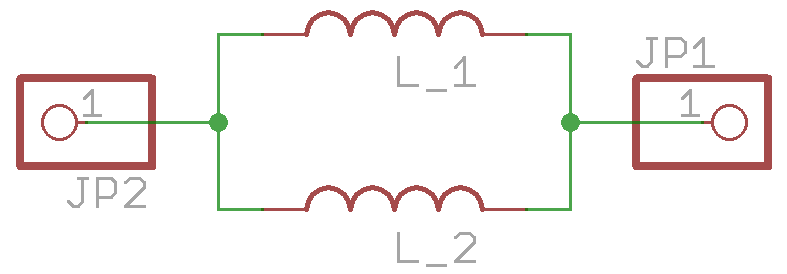
\includegraphics[width=1\textwidth,height=.35\textheight,keepaspectratio]{e06/L_Parallel.png}
      \caption{Spulen in einer Parallelschatung}
    \end{figure}
  \end{center}
  \begin{block}{Parallelschaltung}
    $\frac{1}{L_{gesamt}} = \frac{1}{L_1} + \frac{1}{L_2} + \frac{1}{L_3} + \cdots$\\
    $L_{ges} = \cfrac{1}{\frac{1}{L_1} + \frac{1}{L_2} + \frac{1}{L_3} + \cdots}$
  \end{block}
\end{frame}


\section*{Transformator}

\begin{frame}
  \frametitle{Transformator}
  \begin{center}
    \begin{figure}
      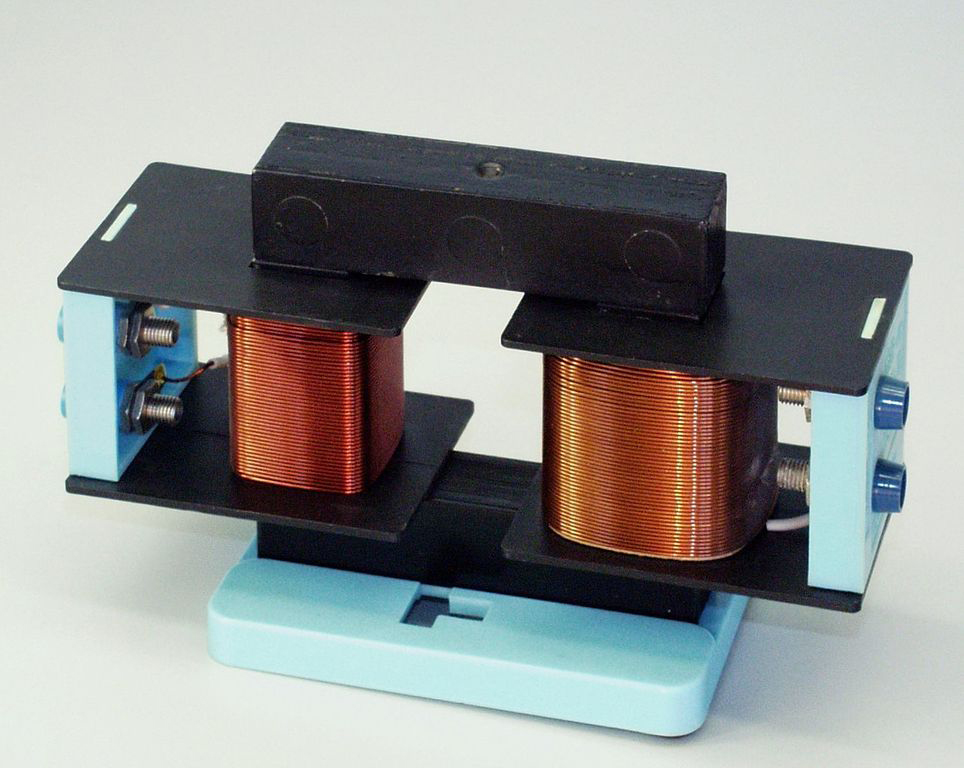
\includegraphics[width=\textwidth,height=.75\textheight,keepaspectratio]{e06/trafo-Real.jpg}
      \attribcaption{Transformator}{Zátonyi Sándor (ifj.), Fizped}{https://commons.wikimedia.org/wiki/File:Trafo_6.jpg}{\ccbysa}
    \end{figure}
  \end{center}
\end{frame}

\begin{frame}
  \frametitle{Transformator}
  \begin{center}
    \begin{figure}
      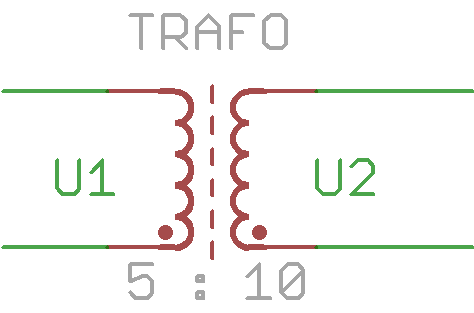
\includegraphics[width=\textwidth,height=.3\textheight,keepaspectratio]{e06/Trafo.png}
      \caption{Transformator}
    \end{figure}
  \end{center}
  \begin{block}{Übertrager}
    \begin{center}
      $\cfrac{N_1}{N_2} = \cfrac{U_1}{U_2}$
    \end{center}
  \end{block}
  Die Spannungen verhalten sich analog zu den Windungszahlen der Spulen eines Transformators.
\end{frame}

%\begin{frame}
%  \frametitle{Prüfungsfrage}
%
%  \begin{center}
%    \begin{tabular}{l||p{.8\textwidth}}
%      \textbf{TC306} & \textbf{Ein Trafo liegt an 230 Volt und gibt $11,5V$ ab. Seine Primärwicklung hat 600 Windungen. Wie groß ist seine Sekundärwindungszahl?} \\\hline\hline
%      A & 20 Windungen\\ \hline
%      B & 180 Windungen \\ \hline
%      C \only<2>\checkmark &  30 Windungen \\ \hline
%      D & 520 Windungen \\ \hline
%    \end{tabular}
%  \end{center}
%\end{frame}


\section*{Referenzen}

\begin{frame}
  \frametitle{Referenzen/Links}

  \footnotesize
  \begin{itemize}
    \item Moltrecht E 06: \\
      \url{https://www.darc.de/der-club/referate/ajw/lehrgang-te/e06/}
    \item WP Trafo: \\
      \url{https://de.wikipedia.org/wiki/Transformator}
    \item WP Spule: \\
      \url{https://de.wikipedia.org/wiki/Spule_(Elektrotechnik)}
  \end{itemize}

\end{frame}

% Hier könnte noch eine Kontaktfolie stehen

\end{document}

